%xelatex -shell-escape -output-directory=bin ergasia.tex
\documentclass{assignment}


\usepackage{pdflscape}
\usepackage{enumerate} % Για την χρησιμοποίηση roman enumerate
\usepackage{paralist} % για το περιβάλλον inparaenum που είναι οι λίστες μέσα στο κείμενο.

\title{Πληροφοριακό σύστημα για online βιβλιοθήκη}
\date{Αθήνα, 2015}

\author{Αναγνωστόπουλος Βασίλης - Θάνος (ΜΠΠΛ 13002) \\
        Βιδάλης Γιάννης (ΜΠΠΛ 13085) \\
        Λιόλης Γιώργος  (ΜΠΠΛ 13049) \\
        Χρόνη Ειρήνη    (ΜΠΠΛ 13083)  }

\begin{document}

\maketitle
% Να σκεφτώ τί αλλαγές θέλω να κάνω με τις αριθμήσεις και άμα θέλω να κάνω.
% Να σκεφτώ να τις ενσωματώσω και στο assignment.cls

\setcounter{page}{1} 
\pagenumbering{roman}

\pagestyle{plain}
\tableofcontents
\listoftables
\listoffigures
\renewcommand\listoflistingscaption{Κατάλογος πηγαίου κώδικα}
\renewcommand\listingscaption{Πηγαίος κώδικας}
\listoflistings
\newpage

%\pagestyle{headings}
%\pagestyle{fancy}
\setcounter{page}{1} 
\pagenumbering{arabic}

\section{Εισαγωγή}

Η εργασία αυτή έχει ως σκοπό την σχεδίαση και ανάλυση ενός πληροφοριακός συστήματος. Συγκεκριμένα η παρούσα αναφορά περιγράφει την βασική λειτουργικότητα και τις σχεδιαστικές αποφάσεις που αφορούν την υλοποίηση του Πληροφοριακού Συστήματος (Π.Σ.) για την δημιουργία μίας ηλεκτρονικής βιβλιοθήκης. Θα παρουσιαστούν οι λειτουργικές και οι μη λειτουργικές απαιτήσεις του συστήματος, το περιβάλλον το οποίο θα χρησιμοποιείται καθώς και οι χρήστες του. Στην συνέχεια θα γίνει μοντελοποίηση του συστήματος με την βοήθεια των διαγραμμάτων της \en{uml} (π.χ. διαγραμμάτων κλάσεων, διαγραμμάτων ροής και περιπτώσεων χρήσης, κ.λ.π.) και έπειτα θα ακολουθήσει η υλοποίηση του συστήματος.

\subsection{Περιβάλλον του έργου}

Η παρούσα μελέτη είναι μελέτη σκοπιμότητας για την οργάνωση και τη λειτουργία της δημοτικής βιβλιοθήκης του Καλλικρατικού Δήμου Διονύσου, η οποία από εδώ και πέρα απλώς θα καλείται απλώς ως "βιβλιοθήκη". 

Η βιβλιοθήκη θα οργανωθεί σύμφωνα με τα σύγχρονα πρότυπα έτσι ώστε να ικανοποιεί πλήρως τις ανάγκες των χρηστών της και την οργάνωση της συλλογής της βιβλιοθήκης σύμφωνα με τους Διεθνείς κανόνες καταλογογράφησης και ευρετηρίασης, τη δημιουργία ηλεκτρονικού Δημοσίου Καταλόγου Ανοικτής Πρόσβασης και την παροχή σύγχρονών υπηρεσιών πληροφόρησης στους χρήστες της, την ορθολογική οργάνωση του διαθέσιμου χώρου λειτουργίας της και γενικότερα τη διαχείριση των διαθέσιμων πόρων για την βελτιστοποίηση των στόχων της.

Ο σχεδιασμός της βιβλιοθήκης θα πρέπει να είναι ευέλικτος και θα πρέπει

\begin{itemize}
\item να επιτρέπει την πλήρη αξιοποίηση των προτύπων οργάνωσης και λειτουργίας, καθώς και των προϊόντων τεχνολογίας και πληροφόρησης, 
\item υιοθέτηση νέων προτύπων στις μεθόδους επεξεργασίας, οργάνωσης, αποθήκευσης και διάδοσης των πληροφοριών,
\item χρησιμοποιήση νέων προϊόντων τεχνολογίας και 
\item παροχή νέων υπηρεσιών πληροφόρησης
\end{itemize}

\subsection{Περιγραφή του προβλήματος και των εναλλακτικών λύσεων}

Ο δήμος Διονύσου για την επιμόρφωση των κατοίκων του Δήμου προωθεί την δημιουργία μίας νέας δημοτικής βιβλιοθήκης. Μία βιβλιοθήκη είναι ένας οργανισμός, ο οποίος λειτουργεί ως κρίκος σύνδεσης των μελών μίας κοινότητας με τις γνώσεις και τις πληροφορίες που χρειάζονται. Τα μέλη της συγκεκριμένης βιβλιοθήκης είναι όλοι οι κάτοικοι του Δήμου και σκοπός της είναι:

\begin{enumerate}
\item να βοηθήσει στην επιμόρφωση των κατοίκων της περιοχής
\item να συμβάλει στην παροχή πληροφοριών που διαφορετικά θα ήταν δυσπρόσιτες στους κατοίκους
\end{enumerate}

Οι εναλλακτικές λύσεις είναι:

\begin{enumerate}
\item να μην γίνει καμία ενέργεια, πράγμα που θα οδηγούσε στην στασιμότητα της επιμόρφωσης των κατοίκων.
\item να συνεχιστεί η κατασκευή της βιβλιοθήκης, πράγμα που θα οδηγήσει στην περαιτέρω επιμόρφωση των κατοίκων
\end{enumerate}


Ακόμα, με την διείσδυση των νέων τεχνολογιών στην καθημερινότητα, οι άνθρωποι χρησιμοποιούν όλο και περισσότερο το διαδίκτυο για την πραγματοποίηση απλών καθημερινών διαδικασιών. Παρά το γεγονός ότι η χρήση του internet παραμένει χαμηλή στη Ελλάδα συγκριτικά με την Ευρώπη, σχεδόν ένας στους πέντε Έλληνες (ποσοστό 20,08\%) χρησιμοποιεί πια το διαδίκτυο, ενώ το 17,9\% του πληθυσμού το χρησιμοποιεί τακτικά τουλάχιστον μια φορά την εβδομάδα. Οι νεαρότερες ηλικιακά ομάδες (16-24 ετών: 42\%, 25-34 ετών: 30\%) και οι κάτοικοι των αστικών πόλεων με ανώτερη μόρφωση, αποτελούν με σημαντική διαφορά τις ομάδες πληθυσμού με την υψηλότερη πρόσβαση \cite{infosoc}. 

Βασισμένοι στα παραπάνω, θεωρείται σημαντικό για την προώθηση της νέας δημοτικής βιβλιοθήκης της να αναπτυχθεί ένα σύστημα λογισμικού για την ενοικίαση βιβλίων μέσω διαδικτύου.

\subsection{Σκοπός και στόχος του Π.Σ.}

Σκοπός της συγκεκριμένης μελέτης είναι η υλοποίηση ενός Π.Σ. που αποσκοπεί στην κατασκευή μίας βιβλιοθήκης που η διαχείριση της θα γίνεται με ηλεκτρονικούς τρόπους. Ταυτόχρονα το νέο Π.Σ. θα βοηθήσει στην οργάνωση της βιβλιοθήκης. Το Π.Σ. αναμένεται να αποφέρει οφέλη στους τομείς:

\begin{itemize}
\item της διαφήμισης, μίας και η ιστοσελίδα θα βοηθήσει στην προώθηση της δημοτικής βιβλιοθήκης
\item της εξυπηρέτησης των χρηστών, μίας και οι δημότες δεν θα πρέπει να περιμένουν στην σειρά για την απόκτηση θέσης για την κράτηση ενός βιβλίου.
\item της οργάνωσης της βιβλιοθήκης, μίας και θα δημιουργηθεί ένα αυτόματο σύστημα επεξεργασίας της διαθεσιμότητας των βιβλίων
\item της μείωση του κόστους, μίας και θα μειωθούν οι εργαζόμενοι οι οποίοι θα πρέπει να απασχολούνται στην δημοτική βιβλιοθήκη. 
\end{itemize}

Η επιτυχία του έργου θα κριθεί κυρίως από το εύρος χρήσης του και από την αξιοποίηση των εξειδικευμένων δυνατοτήτων του, που αποσκοπούν κύρια στην αυτοματοποίηση του συστήματος.

Μετά την ολοκλήρωση του έργου του Π.Σ. θα ωφεληθούν άμεσα:

\begin{itemize}
\item οι εργαζόμενοι της βιβλιοθήκης μιας και θα απλοποιηθεί η διαδικασία για την λειτουργία της 
\item οι κάτοικοι που χρησιμοποιούν την βιβλιοθήκη, μίας και η βιβλιοθήκη θα είναι πιο εύκολα προσβάσιμη. 
\end{itemize}

\subsection{Υφιστάμενη κατάσταση}

Η βιβλιοθήκη στην τωρινή της κατάσταση διατηρεί ηλεκτρονική σελίδα, η οποία όμως σαν στόχο έχει την ενημέρωση των δημοτών για τον κανονισμό λειτουργίας της, το ωράριο και για τις εκδηλώσεις που διοργανώνει. Η δυνατότητα αναζήτησης βιβλίων στον κατάλογο της και η αίτηση δανεισμού δεν περιέχονται στις λειτουργίες της. 

\subsection{Βασικές οντότητες και εμπλεκόμενοι στην υλοποίηση του έργου}

Οι βασικοί εμπλεκόμενοι στην υλοποίηση του έργου είναι οι χρήστες και οι υπάλληλοι της βιβλιοθήκης. Το άμεσο περιβάλλον του έργου και το επιχειρηματικό μοντέλο παριστάνεται στο σχήμα \ref{fig:entities}. Οι οντότητες αυτές αναλύονται παρακάτω. 

\begin{figure}
\begin{center}
\resizebox*{\textwidth}{!}{%
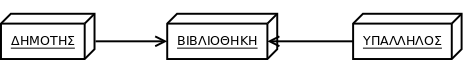
\includegraphics{images/Entities.png}}
\caption{Οι βασικές οντότητες του Πληροφορικού Συστήματος}
\label{fig:entities}
\end{center}
\end{figure}

Ως χρήστες ορίζονται όλοι όσοι επιθυμούν να δανειστούν κάποιο βιβλίο. Ως υπάλληλοι ορίζονται όλοι οι υπάλληλοι της βιβλιοθήκης, είτε μόνιμοι είτε συμβασιούχοι. Οι υπάλληλοι αυτοί έχουν αναλάβει την συντήρηση της βιβλιοθήκης και θα πρέπει να εξυπηρετούν του χρήστες της, να εξοπλίζουν την βιβλιοθήκη με νέα βιβλία καθώς και να προωθούν την βιβλιοθήκη.

Η βασική απαίτηση του συστήματος (δηλαδή η επιχειρηματική απαίτηση του Π.Σ.) είναι η γεφύρωση του χάσματος μεταξύ των χρηστών και των υπάλληλων με σκοπό την αύξηση της χρηστικότητας της βιβλιοθήκης.

Στις παρακάτω ενότητες θα περιγραφούν οι προδιαγραφές και οι περιορισμοί στους οποίους θα πρέπει να συμμορφώνεται το υπό μελέτη πληροφοριακό σύστημα. Θα πρέπει να διασφαλίζει ότι θα ικανοποιούνται οι ανάγκες των ενδιαφερόμενων και για να γίνει αυτό θα πρέπει να οριστούν με ακρίβεια οι λειτουργικές και οι μη λειτουργικές απαιτήσεις.

Θα παρουσιαστούν οι απαιτήσεις που πρέπει να ικανοποιεί το Πληροφοριακό Σύστημα, οι βασικές λειτουργίες που πρέπει να επιτελεί, οι πληροφορίες που πρέπει να αποθηκεύει και οι κανόνες που επιβάλλονται από την λειτουργία του συστήματος.

\subsection{Μοντέλο διαδικασία υλοποίησης και ανάπτυξης του λογισμικού}

Ο κύκλος ζωής του λογισμικού προτείνεται να είναι επαναληπτικός \cite{virvou_uml} και γι` αυτό το λόγο προτείνεται να χρησιμοποιηθεί η διαδικασία Unified της Rational (αγγλ. \en{Rational Unified Process - RUP}).

Η διαδικασία \en{Rational Unified Process (RUP)} αποτελείται από ένα σύνολο οδηγιών σχετικά με τις τεχνικές και οργανωτικές απόψεις της ανάπτυξης λογισμικού, οι οποίες συνοψίζονται παρακάτω \cite{wazlawick2014object}:

\begin{description}
\item[Καθοδήγηση από τις περιπτώσεις χρήσης:] η ανάπτυξη σχεδιάζεται και οργανώνεται χρησιμοποιώντας έναν κατάλογο από περιπτώσεις χρήσεις. 
\item[Καθοδήγηση με βάση την αρχιτεκτονική:] Η διαδικασία ανάπτυξης οδηγεί στην κατασκευή μία αρχιτεκτονικής συστήματος που επιτρέπει την εφαρμογή των απαιτήσεων. Αυτή η αρχιτεκτονική βασίζεται στον προσδιορισμό μίας επαναληπτικής δομής ή οποία βασίζεται στο εννοιολογικό μοντέλο του συστήματος.
\item[Επαναληπτική: ] Η ανάπτυξη χωρίζεται σε επαναλήψεις ή κύκλους ανάπτυξης. Σε κάθε επανάληψη, νέα χαρακτηριστικά προστίθενται στο σύστημα ή διορθώνονται ήδη υλοποιημένα, με αποτέλεσμα το σύστημα να γίνεται πιο πλήρες και πιο κοντά στο τελικό επιθυμητό σύστημα.
\item[Αποφυγή του κινδύνου: ] Τα στοιχεία που ενέχουν τον μεγαλύτερο κίνδυνο για το έργο απευθύνονται πιο νωρίς.  
\end{description}

Ο κύκλος ζωής λογισμικού όπως προτείνεται από την RUP φαίνεται στο σχήμα \ref{fig:rup_cycle}.

\begin{figure}
\begin{center}
\resizebox*{\textwidth}{!}{
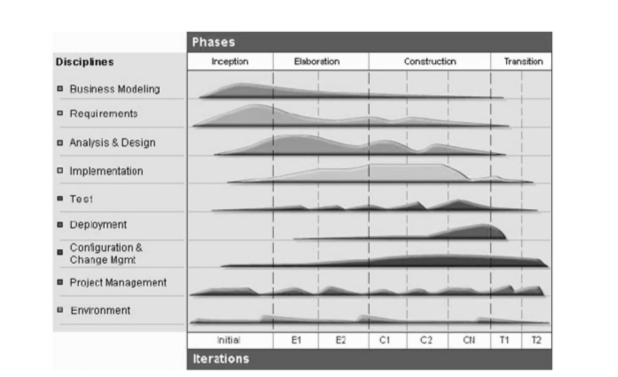
\includegraphics{images/rup.png}}
\caption{Κύκλος ζωής ανάπτυξης λογισμικού με την RUP \cite{wazlawick2014object}}
\label{fig:rup_cycle}
\end{center}
\end{figure}

\section{Φάση: Έναρξη}
\label{section:inception}

Η φάση της έναρξης (αγγλ. \en{inception}) είναι η πρώτη φάση της Unified Process (UP), στην οποία οι κύριες απαιτήσεις του έργου ανακαλύπτονται και έκταση του συστήματος γίνεται κατανοητή. Το προϊόν της φάσης αυτής είναι ένα προκαταρκτικό εννοιολογικό μοντέλο, ανάλυση απαιτήσεων του προκαταρκτικού εννοιολογικού μοντέλου, συνήθως με την μορφή ενός καταλόγου των περιπτώσεων υψηλού επιπέδου χρήσης και ένα χρονοδιάγραμμα (που σε αυτή την εργασία κρίνεται σκόπιμο να μην υλοποιηθεί)\cite{wazlawick2014object}. Ακόμα θα δοθεί ένα πρώτο διάγραμμα τάξεων το οποίο θα δείχνει την υλοποίηση των περιπτώσεων χρήσης.

\subsection{Ανάλυση Απαιτήσεων Πληροφοριακού Συστήματος}

Η ανάλυση απαιτήσεων περιλαμβάνει τις εργασίες για τον καθορισμό των αναγκών ή των προϋποθέσεων που χρειάζονται για την ολοκλήρωση ενός προϊόντος (στην συγκεκριμένη περίπτωση του πληροφοριακού συστήματος). Στην ανάλυση απαιτήσεων λαμβάνονται υπόψιν οι ενδεχόμενες αντικρουόμενες απαιτήσεις των διαφόρων μερών ενώ ταυτόχρονα αναλύονται και τεκμηριώνονται οι τυχόν απαιτήσεις του προϊόντος \cite{wiki:requirement_analysis}. Για να είναι επιτυχές ένα πληροφοριακό σύστημα θα πρέπει να είναι προσαρμοσμένο στις ανάγκες, απαιτήσεις, αλλά και προσδοκίες του τελικού χρήστη. Αυτό σημαίνει ότι το ζητούμενο είναι, τί πραγματικά επιθυμεί ο χρήστης, τί ακριβώς περιμένει από το σύστημα και πόσο φιλικό είναι αυτό σε αυτόν και κατά πόσο ικανοποιεί τους σκοπούς για τους οποίους υλοποιήθηκε.  

Οι απαιτήσεις λογισμικού περιλαμβάνουν 3 διαφορετικά επίπεδα \cite{triadis}:

\begin{itemize}
\item Επιχειρηματικές απαιτήσεις
\item Απαιτήσεις χρηστών
\item Λειτουργικές απαιτήσεις
\end{itemize}

Οι επιχειρηματικές απαιτήσεις αντιπροσωπεύουν τους υψηλού επιπέδου στόχους του οργανισμού ή των πελατών που ζητούν το σύστημα. Ορίζουν τον σκοπό και το πεδίο εφαρμογής του νέου συστήματος λογισμικού και περιγράφουν γιατί ο οργανισμός θέλει να εφαρμόσει το σύστημα.  \cite{triadis}.

Οι απαιτήσεις των χρηστών περιγράφουν τους στόχους των χρηστών ή τα καθήκοντα που θα έχουν οι χρήστες στο προϊόν. Οι ανάγκες των χρηστών περιγράφουν τί θα κάνουν οι χρήστες μέσα στο σύστημα. Θα πρέπει να ευθυγραμμίζονται με τις επιχειρηματικές απαιτήσεις. \cite{triadis}

Τέλος οι λειτουργικές απαιτήσεις καθορίζουν την λειτουργικότητα του λογισμικού που πρέπει να φτιάξουν τα μέλη της ομάδας ανάπτυξης έτσι ώστε το προϊόν να επιτρέπει στους χρήστες να εκπληρώνουν τα καθήκοντα τους καλύπτοντας έτσι τις επιχειρησιακές απαιτήσεις \cite{triadis}.

Η ανάλυση απαιτήσεων συντελεί στην καλή οργάνωση και εκτέλεση του έργου, που με τη σειρά τους εξασφαλίζουν τη λειτουργικότητά του για όλες τις εμπλεκόμενες πλευρές. Στο τέλος, τα οφέλη αυτά έχουν άμεσο αντίκρισμα στη μείωση του κόστους, τόσο για την επιχείρηση που υλοποιεί το έργο όσο και για τον πελάτη που θα το χρησιμοποιήσει \cite{kepa:requirement_analysis}.

Οι λειτουργικές απαιτήσεις μαζί με τα χαρακτηριστικά ποιότητας και άλλες μη λειτουργικές απαιτήσεις δημιουργούν την προδιαγραφή των απαιτήσεων λογισμικού \cite{triadis}. 

Η παρούσα αναφορά περιγράφει την βασική λειτουργικότητα και τις σχεδιαστικές αποφάσεις που αφορούν την υλοποίηση του Π.Σ. της δημοτικής βιβλιοθήκης.

\subsection{Αρχιτεκτονική}

Οι γενικές αρχές, σε λειτουργικό και τεχνολογικό επίπεδο, που θα διέπουν το Π.Σ. που θα αναπτυχθεί είναι:

\begin{enumerate}
\item Συστήματα "ανοικτής" αρχιτεκτονικής (αγγλ. \en{open architecture}). Είναι δηλαδή υποχρεωτική η χρήση ανοικτών προτύπων που θα διασφαλίζουν ανεξαρτησία από συγκεκριμένο προμηθευτή και:

  \begin{itemize}
    \item ομαλή συνεργασία και λειτουργία μεταξύ των επιμέρους Υποσυστημάτων του πληροφοριακού συστήματος,
    \item δικτυακή συνεργασία μεταξύ εφαρμογών ή/και συστημάτων τα οποία βρίσκονται σε διαφορετικά υπολογιστικά συστήματα,
    \item επεκτασιμότητα των υποσυστημάτων, χωρίς αλλαγές στη δομή και αρχιτεκτονική τους, για την αντιμετώπιση των μεταβαλλόμενων / αυξανόμενων αναγκών
    \item εύκολη επέμβαση στη λειτουργικότητα των υποσυστημάτων (συντηρησιμότητα - \en{maintainability})
    \item ύψιστη διασφάλιση των δεδομένων.
  \end{itemize}

\item Αρθρωτή αρχιτεκτονική του συστήματος, ώστε να επιτρέπονται μελλοντικές επεκτάσεις και αντικαταστάσεις, ενσωματώσεις, αναβαθμίσεις ή αλλαγές διακριτών τμημάτων λογισμικού ή εξοπλισμού.

\item Εξασφάλιση πλήρους λειτουργικότητας μέσω του εσωτερικού δικτύου (αγγλ. \en{intranet}) και του διαδικτύου (αγγλ. \en{internet}) όπου αυτό απαιτείται.

\item Χρήση γραφικού περιβάλλοντος λειτουργίας (αγγλ. \en{GUI}) του χρήστη για την αποδοτική χρήση του Π.Σ. και την ευκολία εκμάθησης τους.

\item Ενσωμάτωση στο Π.Σ. άμεσης υποστήριξης βοήθειας (αγγλ. \en{online help}) και οδηγιών στην ελληνική γλώσσα, προς τους χρήστες ανά διαδικασία ή/και οθόνη.

\item Μηνύματα λαθών (αγγλ. \en{error messages}) στην ελληνική γλώσσα και ειδοποίηση των χρηστών με όρους οικείους προς αυτούς.

\item Tήρηση από το Π.Σ. στοιχείων auditing για ιχνηλάτηση
ενεργειών χρηστών.

\item Διασφάλιση της πληρότητας, ακεραιότητας, εμπιστευτικότητας και ασφάλειας των δεδομένων των Υποσυστημάτων κατά τη χρήση και τη δικτυακή διακίνησή τους.

\item Τεκμηρίωση του Π.Σ. μέσω της αναλυτικής περιγραφής της βάσης δεδομένων. Σύνταξη τεχνικών εγχειριδίων του συστήματος και των εργαλείων διαχείρισης (αγγλ. \en{system manuals}), καθώς και λεπτομερή εγχειρίδια λειτουργίας του συστήματος (αγγλ. \en{operation manuals} ) και υποστήριξης των χρηστών (αγγλ. \en{user manuals}).

\end{enumerate}

\subsection{Χρήστες}

Το πληροφορικό σύστημα θα έχεις ως χρήστες τους υπαλλήλους της δημοτικής βιβλιοθήκης αλλά και τους κατοίκους του δήμου. Βασική απαίτηση του συστήματος είναι οργάνωση της βιβλιοθήκης έτσι ώστε να μπορεί να διαχειρίζεται τα βιβλία που θα έχει και να τα δανείζει στους κατοίκους του δήμου χωρίς να υπάρχει κίνδυνος απώλειας τους.

\subsection{Λειτουργικές απαιτήσεις}

Οι λειτουργικές απαιτήσεις είναι οι κύριες δυνατότητες του συστήματος. Αναπαριστούν το "τί" θα κάνει το σύστημα που θα αναπτυχθεί, χωρίς να αναφέρονται στον τρόπο με τον οποίο ("πως") το σύστημα θα το κάνει \cite{triadis}.

\subsubsection{Λειτουργικότητα και διαγράμματα περίπτωσης χρήσης}
\label{subsubsection: business_use_case}

Η λειτουργικότητα ενός συστήματος μετράται από το πόσο καλά ικανοποιεί τις λειτουργικές απαιτήσεις των ενδιαφερόμενων. Το Π.Σ. για τον δανεισμό των βιβλίων υλοποιεί τη απαιτούμενη μηχανογράφηση για την βιβλιοθήκη. Βασική απαίτηση από το Π.Σ. είναι η αποθήκευση των απαιτούμενων πληροφοριών για τον δανεισμό των βιβλίων. Τέλος μέσω του Π.Σ. θα πρέπει να μπορούν να γίνονται τα εξής:

\begin{itemize}
\item Αυτόματη ενημέρωση της κεντρικής ιστοσελίδας του Π.Σ. ανάλογα με το τις πληροφορίες που εισάγουν οι διαχειριστές του Π.Σ. .
\item Αυτόματη δημιουργία λογαριασμών, μέσω των οποίων οι δημότες θα μπορούν να βλέπουν ποια βιβλία είναι διαθέσιμα.
\item Το σύστημα θα πρέπει να επιτρέπει στους χρήστες να ενημερώνουν τις προσωπικές τους πληροφορίες.
\item Το σύστημα θα πρέπει να μπορεί να παρέχει πληροφορίες για τα βιβλία.
\item Θα πρέπει να επιτρέπει την επικοινωνία μεταξύ των δημοτών και των υπαλλήλων της βιβλιοθήκης. 
\item Το σύστημα θα πρέπει να κρατά το ιστορικό των δανεισμών ενός δημότη.
\item Το σύστημα θα πρέπει να επιτρέπει την δημιουργία στατιστικών στοιχείων για τα βιβλία.
\item Το σύστημα θα πρέπει να βοηθάει στην προώθηση της δημοτικής βιβλιοθήκης μέσω της κεντρικής ιστοσελίδας.
\end{itemize}

Όλες οι απαιτούμενες λειτουργικότητες υψηλού επιπέδου από το Π.Σ. φαίνονται στο UML διάγραμμα χρήσης (αγγλ. \en{use case diagram}) (βλ. σχήμα \ref{fig:business_activity_diagram}). Στην ενότητα \ref{section: Elaboration} θα αναπτυχθούν σε uml διάγραμμα και οι υπόλοιπες λειτουργικότητες που περιγράφονται σε αυτή την ενότητα

Τα διαγράμματα περιπτώσεων - χρήσης (αγγλ. \en{Use Case Diagrams}) περιγράφουν τη συμπεριφορά ενός συστήματος από την οπτική γωνία των χρήστών. Επιτρέπουν τον ορισμό των ορίων του συστήματος και του περιβάλλοντος \cite{virvou_uml}. Οι συμβολισμοί που χρησιμοποιούνται στα διαγράμματα περιπτώσεων - χρήσης φαίνονται στον πίνακα \ref{table:uml_use_case}. 

\begin{table}
\begin{center}
  \begin{tabular}{|m{0.20\textwidth}|m{0.60\textwidth}|}
    \hline
     %\vspace{0.3cm}
     \center{
     \resizebox*{0.10\textwidth}{!}{
     
\includegraphics{images/use_case_user.png}}}
     & Ο ενεργοποιός του συστήματος. Ο ενεργοποιός αναπαριστά έμα ρόλο που παίζεται από ένα άτομο ή πράγμα που αλληλεπιδρά με το σύστημα \cite{virvou_uml}. \\ \hline

     \vspace{0.3cm}
     \resizebox*{0.20\textwidth}{!}{
     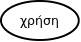
\includegraphics{images/use_case_case.png}}
     & Περίπτωση χρήσης. Περιγράφει τις δυνατές αλληλεπιδράσεις με το σύστημα \cite{virvou_uml}. \\ \hline

     \vspace{0.3cm}
     \center
     \resizebox*{0.20\textwidth}{!}{
     
\includegraphics{images/use_case_communication.png}}
     & Η σχέση <<communicates>>. Η σχέση αυτή ορίζεται μεταξύ περιπτώσεων χρήσης και σημαίνει ότι ένα στιγμιότυπο της πηγής (περίπτωσης χρήσης) συμπεριλαμβάνει τη συμπεριφορά του στόχου (περίπτωση χρήσης) \cite{virvou_uml}. \\ \hline

     \vspace{0.3cm}
     \resizebox*{0.20\textwidth}{!}{
     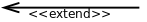
\includegraphics{images/use_case_extend.png}}
     & Η σχέση <<extend>>. Δείχνει προαιρετική συμπεριφορά μίας περίπτωση χρήσης \cite{virvou_uml}. \\ \hline

     \vspace{0.3cm}
     \resizebox*{0.20\textwidth}{!}{
     
\includegraphics{images/use_case_include.png}}
     & Η σχέση <<include>>. Χρησιμοποιείται για να δείξει λειτουργικότητα που τη μοιράζονται πολλές περιπτώσεις χρήσης \cite{virvou_uml}. \\ \hline

     \vspace{0.3cm}
     \resizebox*{0.20\textwidth}{!}{
     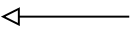
\includegraphics{images/use_case_generalization.png}}
     & Η γενίκευση περιπτώσεων χρήσης. Ο ειδικός ενεργοποιός κληρονομεί τις περιπτώσεις χρήσης του γενικού ενεργοποιού. Το βέλος πρέπει να δείχνει το γενικότερο ενεργοποιό. \cite{virvou_uml}. \\ \hline

     %\vspace{0.3cm}
     \center{
     \resizebox*{0.10\textwidth}{!}{
     
\includegraphics{images/use_case_boundary.png}}}
     & Τα όρια του συστήματος. \\ \hline

  \end{tabular}
\caption{Τα εικονίδια του διαγράμματος περιπτώσεων - χρήσης.}
\label{table:uml_use_case}
\end{center}
\end{table}


\begin{figure}
\begin{center}
\resizebox*{!}{!}{
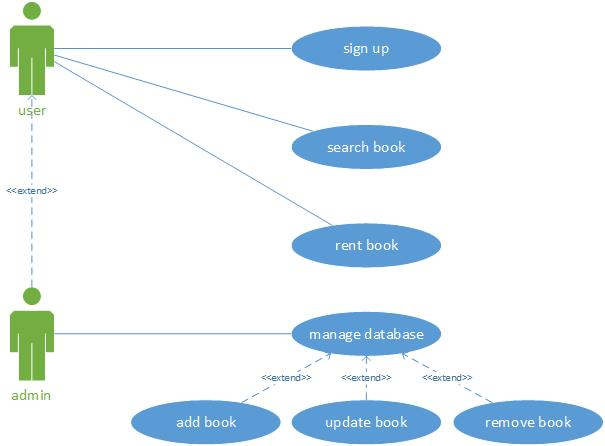
\includegraphics{images/first/UseCaseDiagram.jpg}}
\caption{Διάγραμμα περιπτώσεων - χρήσης (1η φαση)}
\label{fig:activity_diagram(1st)}
\end{center}
\end{figure}

\subsubsection{Διάγραμμα βασικών κλάσεων} 

Ένα διάγραμμα κλάσεων δείχνει την στατική δομή των κλάσεων του συστήματος και των σχέσεων μεταξύ τους. Ένα διάγραμμα κλάσεων συνήθως αποτελείται από:

\begin{itemize}
\item Κλάσεις (αγγλ. \en{Classes})
\item Διαπροσωπίες (αγγλ. \en{Interfaces})
\item Συνεργασίες (αγγλ. \en{Collaborations})
\item Συσχετίσεις (αγγλ. \en{Relationships})
\end{itemize}

Το μοντέλο των κλάσεων χρησιμοποιείται κατά την διάρκεια της ανάλυσης για να περιγράψει τις λειτουργικές απαιτήσεις. Επίσης χρησιμοποιείται κατά την διάρκεια του σχεδιασμού για να περιγράψει το λεξιλόγιο του συστήματος, τις συνεργασίας και το λογικό σχήμα της βάσης δεδομένων \cite{Rumbaugh:2004:UML:993859}.

Στο σχήμα \ref{fig:basic_class_diagramm} φαίνονται οι βασικές κλάσεις καθώς και οι συσχετίσεις μεταξύ τους. Οι βασικές κλάσεις προέκυψαν από το σχήμα \ref{fig:activity_diagram(1st)} καθώς κάθε μία οντότητα του σχήματος θα έπρεπε να αντιστοιχηθεί σε μία κλάση.

Συγκεκριμένα έχουμε την κλάση User που αναπαριστά τους ενεργοποιούς του συστήματος,την κλάση Book που αναπαριστά τα βιβλία και τέλος έχουμε την κλάση Paperbook η αναπαριστά τα "φυσικά" έντυπα των βιβλίων τα οποία ενοικιάζονται στους χρήστες. Από το σχήμα \ref{fig:activity_diagram(1st)} φαίνονται και οι συνδέσεις μεταξύ των κλάσεων.

Στην ενότητα \ref{section: Elaboration} το διάγραμμα κλάσεων θα αναπτυχθεί περισσότερο και σε κάθε κλάση θα προστεθούν και οι μεταβλητές και οι συναρτήσεις τους.

%\begin{landscape}
\begin{figure}
\begin{center}
\resizebox*{!}{!}{
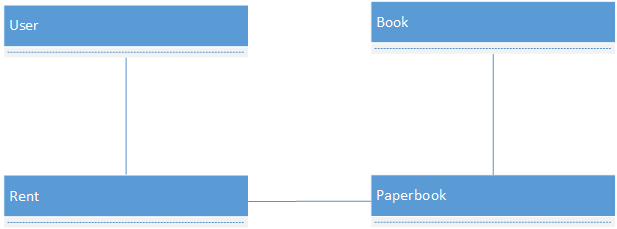
\includegraphics{images/ClassDiagramBasic.png}}
\caption{Το βασικό διάγραμμα κλάσεων}
\label{fig:basic_class_diagramm}
\end{center}
\end{figure}
%\end{landscape}



\subsubsection{Περιορισμοί σχεδιασμού}

Οι σχεδιαστές πρέπει να δημιουργήσουν ένα σύστημα το οποίο θα προσαρμόζεται σε κάποιος περιορισμούς. Αν αυτοί οι περιορισμοί δεν συνυπολογιστούν τότε το σύστημα δεν θα λειτουργεί σωστά και θα καταλήξει σε αποτυχία. 

Το Π.Σ. για την βιβλιοθήκη θα είναι υπεύθυνο για την ενοικίαση των βιβλίων. Επομένως πριν την ενοικίαση ενός βιβλίου θα πρέπει να πραγματοποιείται ένας ελέγχος για την αποφυγή διπλοκρατήσεων.

\subsection{Μη λειτουργικές απαιτήσεις}

Οι μη λειτουργικές απαιτήσεις είναι οι περιορισμοί που τίθενται στις λειτουργικές απαιτήσεις, ή στις απαιτήσεις ποιότητας. Αυτές περιλαμβάνουν πληθώρα ιδιοτήτων συμπεριλαμβάνοντας την επίδοση, τους περιορισμούς πολιτικής, την ασφάλεια, την προστασία προσωπικών δεδομένων, την αξιοπιστία. Καθορίζονται γενικά ως ένα βαθμό μετά την μοντελοποίηση των επιχειρηματικών διαδικασιών. Η μοντελοποίηση των μη λειτουργικών χαρακτηριστικών της επιχείρησης θεωρείται ως ένα δύσκολο πρόβλημα, καθώς η μοντελοποίηση επικεντρώνεται στην λειτουργική συμπεριφορά \cite{triadis}.

Για το Π.Σ. για την βιβλιοθήκη οι μη λειτουργικές απαιτήσεις οι οποίες πρέπει να τηρούνται είναι οι παρακάτω:

\begin{description}
\item[Επίδοση:] Η επίδοση έχει να κάνει με περιορισμούς της ταχύτητας που θα πρέπει να εκτελούνται οι διεργασίες, την ποσότητα των δεδομένων που θα αποθηκεύονται και τους χρόνους απόκρισης του συστήματος \cite{triadis}. Παρακάτω υπάρχουν κάποιοι τέτοιοι περιορισμοί:
\begin{description}
	\item [Απόκριση:] Οι λειτουργίες του εσωτερικού δικτυακού κόμβου πρέπει να έχουν χρόνο απόκρισης εντός ολίγων δευτερολέπτων

	\item [Εκτέλεση απλών ερωτημάτων:] Το 90\% των συναλλαγών θα πρέπει να ολοκληρώνεται σε χρόνο μικρότερο των 2 sec

	\item [Εκτέλεση σύνθετων ερωτημάτων:] To 90\% των συναλλαγών θα πρέπει να ολοκληρώνεται σε χρόνο μικρότερο των 4 sec
\end{description}

\item[Ασφάλεια και προστασία προσωπικών πληροφοριών:] Η ασφάλεια είναι ένας κρίσιμος παράγοντας για όλες τις εφαρμογές. Κατά το σχεδιασμό του Π.Σ. θα πρέπει να ληφθεί ειδική μέριμνα και να δρομολογηθούν οι κατάλληλες δράσεις για:
\begin{itemize}
	\item την προστασία της ακεραιότητας και της διαθεσιμότητας των πληροφοριών
	\item την προστασία των προς επεξεργασία και αποθηκευμένων προσωπικών δεδομένων αναζητώντας και εντοπίζοντας με μεθοδικό τρόπο τα τεχνικά μέτρα και τις οργανωτικο-διοικητικές διαδικασίες
\end{itemize}

\item[Χρηστικότητα - Προσβασιμότητα:] Το σχεδιασμένο σύστημα θα πρέπει να διακρίνεται από υψηλό επίπεδο χρηστικότητας στην οργάνωση και παρουσίαση των ψηφιακών υπηρεσιών που θα παρέχει. Θα πρέπει να λαμβάνονται υπόψιν οι διαφορετικές ομάδες χρηστών κι επομένως τους διαφορετικούς τρόπους εκπλήρωσης της παρεχόμενης λειτουργικότητας χωρίς να μειώνεται η χρηστικότητα των εφαρμογών. Ο σχεδιασμός των εφαρμογών με βασική αρχή την επίτευξη υψηλής χρηστικότητας και εργονομίας είναι κρίσιμος παράγοντας επιτυχίας για το παρόν έργο.

Οι κυριότερες αρχές προς την κατεύθυνση της χρηστικότητας περιλαμβάνουν:
\begin{description}
	\item[Συμβατότητα:] Οι web-εφαρμογές που θα υλοποιηθούν θα πρέπει να είναι προσβάσιμες με τρεις (3) τουλάχιστον, από τους πιο διαδεδομένους
φυλλομετρητές (web browsers).

	\item[Συνέπεια:] Οι εφαρμογές θα πρέπει να έχουν ομοιόμορφη εμφάνιση (κατά το δυνατόν) και να τηρείται συνέπεια στη χρήση των λεκτικών και των συμβόλων. Αντίστοιχη συνέπεια πρέπει να επιδεικνύουν οι οποιεσδήποτε γραφικές απεικονίσεις και οι τοποθετήσεις αντικειμένων. Στο επίπεδο των εφαρμογών και διαδραστικών λειτουργιών, παρόμοιες λεκτικές και λειτουργικές απεικονίσεις πρέπει να αντιστοιχούν σε ανάλογα αποτελέσματα.

	\item [Αξιοπιστία:] Ο χρήστης πρέπει να έχει σαφείς διαβεβαιώσεις δια μέσου της εμφάνισης και συμπεριφοράς του συστήματος ότι οι συναλλαγές του θα διεκπαραιώνονται με ασφάλεια.

	\item[Διαφάνεια:] Ο χρήστης θα πρέπει να "συναλλάσσεται" με το Σύστημα χωρίς να αντιλαμβάνεται τεχνικές λεπτομέρειες ή εσωτερικές διεργασίες διεκπεραίωσης των συναλλαγών.
\end{description}

\item[Συντηρησιμότητα:] Το Π.Σ. θα πρέπει να συντηρείται εύκολα και να επιτρέπονται μελλοντικές επεκτάσεις και αντικαταστάσεις, αναβαθμίσεις ή αλλαγές του Π.Σ. .

\end{description}


\section{Φάση: Εκπόνηση Μελέτης}
\label{section: Elaboration}

Η φάση της εκπόνησης της μελέτης (αγγλ. \en{elaboration phase}) περιλαμβάνει μία πιο λεπτομερή ανάλυση απαιτήσεων, η οποία πραγματοποιείται με την επέκταση των περιπτώσεων χρήσης, δηλαδή, γράφοντας την αλληλουχία των βημάτων που χαρακτηρίζει κάθε μία από τις πιθανές περιπτώσεις τους.  \cite{wazlawick2014object}.  
	
Η φάση της εκπόνησης της μελέτης είναι επαναληπτική. Σε κάθε επανάληψη αναπτύσσονται μία ή περισσότερες περιπτώσεις χρήσης και σε κάθε επανάληψη, οι πληροφορίες που εξάγονται από τις περιπτώσεις χρήσης ενσωματώνονται στο τελικό προϊόν. Στην φάση εκπόνησης αντιμετωπίζονται οι πιο πολύπλοκες περιπτώσεις χρήσεις \cite{wazlawick2014object}.

\subsection{Διαγράμματα περιπτώσεων χρήσης}

Σε συνέχεια από την ενότητα \ref{section:inception} θα συνεχιστεί η ανάλυση απαιτήσεων με εμβάθυνση στις περιπτώσεις χρήσης. Συγκεκριμένα θα αναλυθούν οι ενέργειες που θα πρέπει να εκτελούνται από τους ενεργοποιούς του πληροφοριακού συστήματος 

\begin{landscape}
\begin{figure}
\begin{center}
\resizebox*{!}{!}{
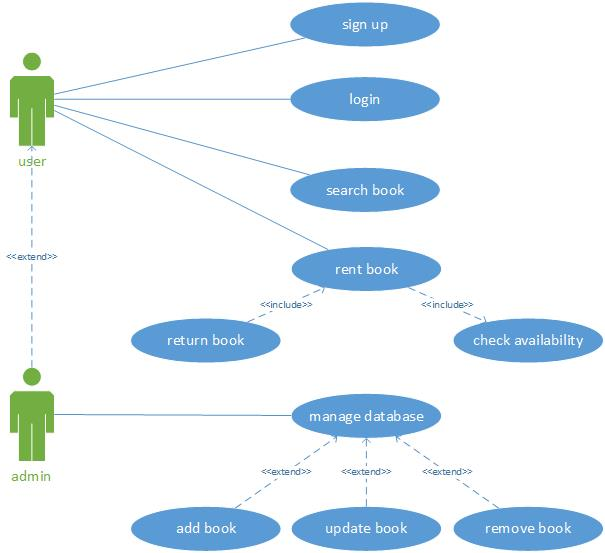
\includegraphics{images/second/UseCaseDiagram.jpg}}
\caption{Το διάγραμμα περιπτώσεων χρήσης των χρηστών}
\label{fig:usecase_diagram_Users}
\end{center}
\end{figure}
\end{landscape}
%http://creately.com/diagram/example/hgmsd6in/Library+information+system
%http://www.programsformca.com/2012/03/uml-diagrams-for-library-management.html

\subsection{Διάγραμμα κλάσεων}

Το διάγραμμα κλάσεων έχει αναπτυχθεί και περιέχει μεταβλητές και συναρτήσεις.

\begin{landscape}
\begin{figure}
\begin{center}
\resizebox*{!}{!}{
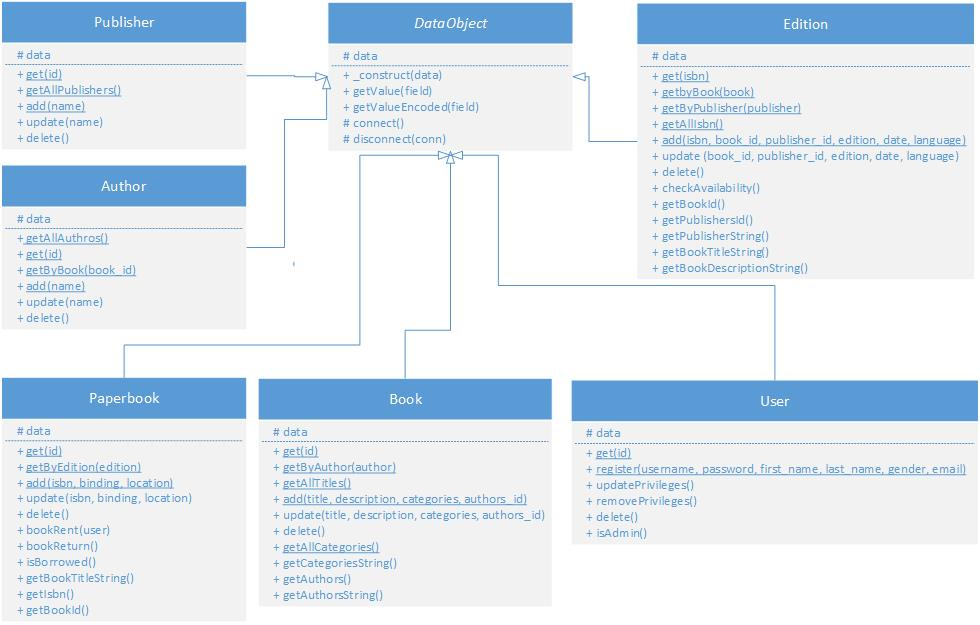
\includegraphics{images/second/ClassDiagram.jpg}}
\caption{Το διάγραμμα κλάσεων}
\label{fig:Class_Diagramm}
\end{center}
\end{figure}
\end{landscape}

\subsection{Διάγραμμα δραστηριότητας}

Ένα διάγραμμα δραστηριότητας αναπαριστά την κατάσταση εκτέλεσης ενός μηχανισμού σαν μία σειρά βημάτων που ομαδοποιούνται σειριακά σαν παράλληλες διακλαδώσεις ροής ελέγχου \cite{virvou_uml}. Βοηθούν στην αποτύπωση λεπτομερειών που δεν φαίνονται στα διαγράμματα των περιπτώσεων χρήσης.

Στο σχήμα \ref{fig:activity_diagram_rent_book_basic} 

\begin{figure}
\begin{center}
\resizebox*{!}{!}{
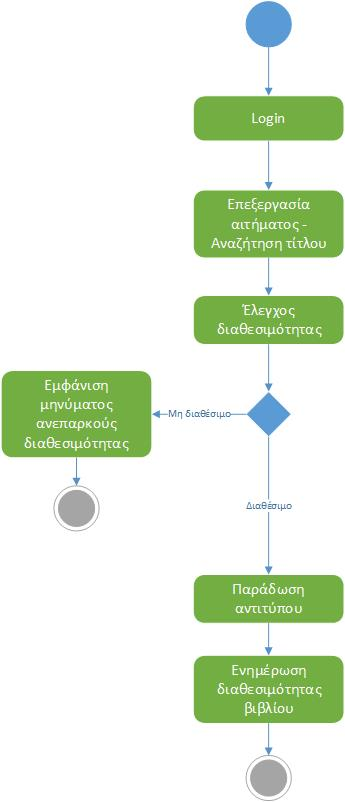
\includegraphics{images/second/ActivityDiagramRentBook.jpg}}
\caption{Το βασικό διάγραμμα δραστηριότητας για την ενοικίαση ενός βιβλίου}
\label{fig:activity_diagram_rent_book_basic}
\end{center}
\end{figure}


\begin{figure}
\begin{center}
\resizebox*{!}{!}{
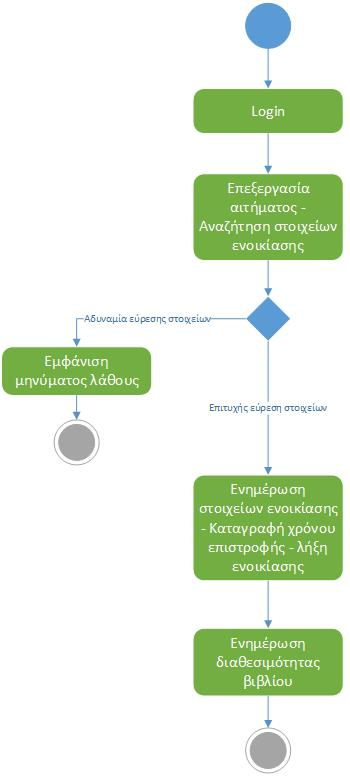
\includegraphics{images/second/ActivityDiagramReturnBook.jpg}}
\caption{Το βασικό διάγραμμα δραστηριότητας για την επιστροφή ενός βιβλίου} 
\label{fig:activity_diagram_return_book_basic}
\end{center}
\end{figure}



\subsection{Διαγράμματα καταστάσεων}

Τα διαγράμματα καταστάσεων αναπαριστούν μηχανές καταστάσεων από την άποψη των καταστάσεων και των μεταβάσεων. Όπως και τα διαγράμματα δραστηριότητας, είναι διαγράμματα συμπεριφοράς, μόνο που αντί να μοντελοποιούν δραστηριότητες, μοντελοποιούν τις καταστάσεις του συστήματος, ενός ενεργοποιού ή μίας οντότητας σε μία συγκεκριμένη στιγμή \cite{virvou_uml,wazlawick2014object}.

\begin{figure}
\begin{center}
\resizebox*{!}{!}{
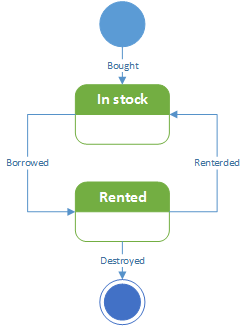
\includegraphics{images/StatechartDiagramBook.png}}
\caption{Διάγραμμα καταστάσεων για ένα βιβλίο} 
\label{fig:statechart_diagram_book}
\end{center}
\end{figure}



\subsection{Διαγράμματα Αντικειμένων}

Τα διαγράµµατα αντικειµένων περιγράφουν ένα σύνολο αντικειµένων καθώς και τις σχέσεις τους µια δεδοµένη χρονική στιγµή και χρησιμοποιούνται για να καταγράψουν στατικές δομές αντικειμένων. Μπορούν να χαρακτηριστούν σαν ένα στιγμιότυπο των διαγραμμάτων κλάσεων. 


\begin{figure}
\begin{center}
\resizebox*{!}{!}{
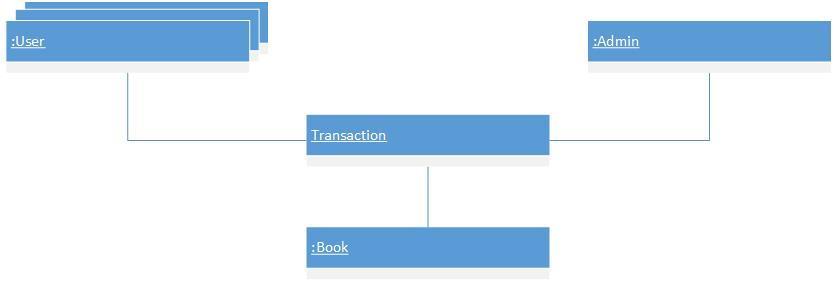
\includegraphics{images/ObjectDiagram.png}}
\caption{Διάγραμμα αντικειμένων} 
\label{fig:object_diagramm}
\end{center}
\end{figure}




\section{Φάση: Κατασκευή}

%During the Construction phase most of the code production and test activities are performed. It is expected that the Elaboration phase produces an architecture sufficiently stable so that its refactoring will be minimized during this phase \cite{wazlawick2014object}.

%The Elaboration and Construction phases are performed in iterations. An iteration may have as an objective developing one or more use cases, implementing change requests, or mitigating selected risks. During an iteration, use cases are expanded and the information learned from them is incrementally incorporated in the product. It is expected that the Elaboration phase deals with the major risks of the system, as well as with the more complex or risky use cases that affect the system architecture significantly. On the other hand, the Construction phase concentrates on producing code for the whole application and implementing change requests \cite{wazlawick2014object}.

\subsection{Διαγράμματα δραστηριότητας}

Σε συνέχεια από την ενότητα \ref{section: Elaboration} έχουμε:

Στο σχήμα \ref{fig:activity_diagram_rent_book_extended} φαίνεται το εκτενές σχήμα του διαγράμματος δραστηριότητας της ενοικίασης ενός βιβλίου και στο σχήμα \ref{activity_diagram_reτurn_book_extended} φαίνεται το εκτενές σχήμα του διαγράμματος δραστηριότητας επιστροφής βιβλίου.

\begin{figure}
\begin{center}
\resizebox*{!}{!}{
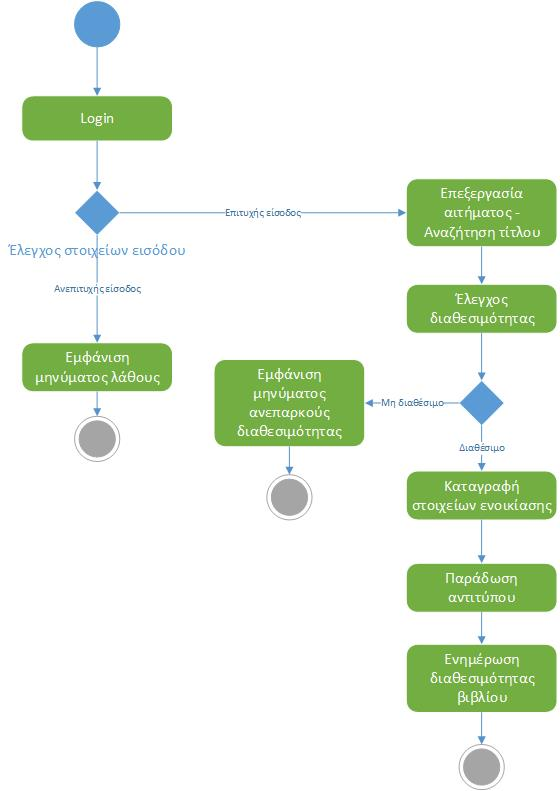
\includegraphics{images/third/ActivityDiagramRentBook.jpg}}
\caption{Το διάγραμμα δραστηριότητας για την ενοικίαση ενός βιβλίου}
\label{fig:activity_diagram_rent_book_extended}
\end{center}
\end{figure}
%https://www.lucidchart.com/pages/activity-diagram-for-library-management-system-UML

\begin{figure}
\begin{center}
\resizebox*{!}{!}{
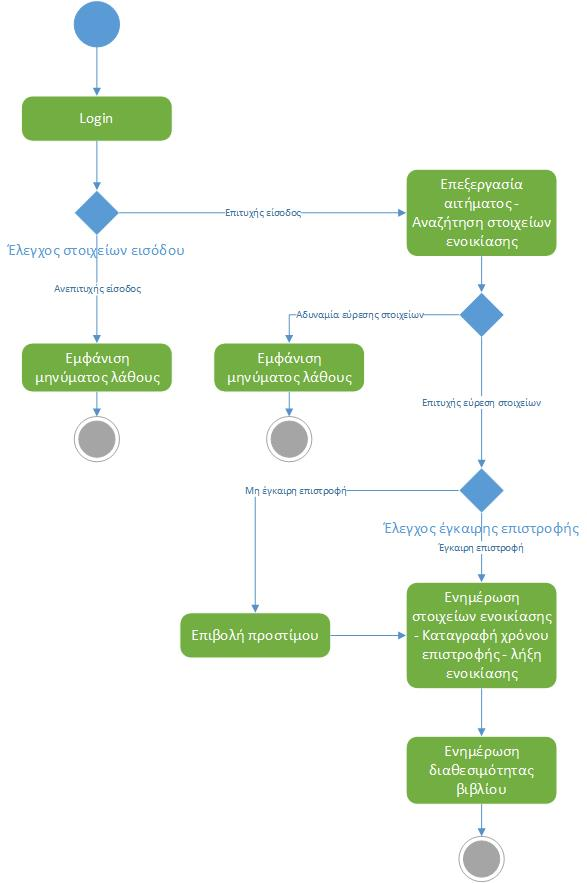
\includegraphics{images/third/ActivityDiagramReturnBook.jpg}}
\caption{Το διάγραμμα δραστηριότητας για την ενοικίαση ενός βιβλίου}
\label{fig:activity_diagram_return_book_extended}
\end{center}
\end{figure}





















\section{Υλοποίηση της Βάσης Δεδομένων}

Σε αυτή την ενότητα περιγράφεται η υλοποίηση της βάσης δεδομένων στο ΣΔΒΔ της MariaDB η οποία είναι ένα fork της MySQL.

\subsection{Εννοιολογικό μοντέλο}

Στο διάγραμμα \ref{fig:ER:diagram} φαίνονται μόνο τα πιο βασικά πεδία. Όλα τα πεδία φαίνονται αναλυτικά στο σχήμα \ref{fig:RelationalModel:diagram}.

\begin{table}
\begin{center}
  \begin{tabular}{|m{0.20\textwidth}|m{0.60\textwidth}|}
    \hline
     \vspace{0.3cm}
     \resizebox*{0.20\textwidth}{!}{
     
\includegraphics{images/entity.jpeg}}
     & Ορθογώνια: οντότητες. \\ \hline

     \vspace{0.3cm}
     \resizebox*{0.20\textwidth}{!}{
     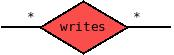
\includegraphics{images/relationship.jpeg}}
     & Ρόμβοι: συσχετίσεις. \\ \hline

     \vspace{0.3cm}
     \resizebox*{0.20\textwidth}{!}{
     
\includegraphics{images/line.jpeg}}
     & Γραμμές: συνδέουν χαρακτηριστικά με οντότητες, οντότητες με συσχετίσεις. \\ \hline

     \vspace{0.3cm}
     %\resizebox*{0.20\textwidth}{!}{
     \center
     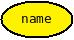
\includegraphics{images/characteristicl.jpeg}%}
     & Ελλείψεις: χαρακτηριστικά. \\ \hline

     \vspace{0.3cm}
     \resizebox*{0.20\textwidth}{!}{
     
\includegraphics{images/characteristicl_many.jpeg}}
     & Διπλές ελλείψεις: πλειότιμα χαρακτηριστικά. \\ \hline

%     \vspace{0.3cm}
     %\resizebox*{0.20\textwidth}{!}{
     \center
%     
\includegraphics{images/characteristicl_many.jpeg}}
%     & Διακεκομμένες ελλείψεις: εξαρτημένα χαρακτηριστικά. \\ \hline

     \vspace{0.3cm}
     %\resizebox*{0.20\textwidth}{!}{
     \center
     
\includegraphics{images/key.jpeg}%}
     & Υπογραμμίσεις: πρωτεύοντα κλειδιά. \\ \hline

     \vspace{0.3cm}
     \resizebox*{0.20\textwidth}{!}{
     
\includegraphics{images/entity_weak.jpeg}}
     & Διπλό ορθογώνιο: Αδύναμο σύνολο οντοτήτων. \\ \hline

     \vspace{0.3cm}
     \resizebox*{0.20\textwidth}{!}{
     
\includegraphics{images/isa.jpeg}}
     & Τρίγωνο: Εξιδίκευση. \\ \hline
  \end{tabular}
\caption{Τα εικονίδια του διαγράμματος οντοτήτων συσχετίσεων.}
\label{table:icons}
\end{center}
\end{table}


\begin{landscape}
\begin{figure}
\begin{center}
\resizebox*{!}{\textwidth}{
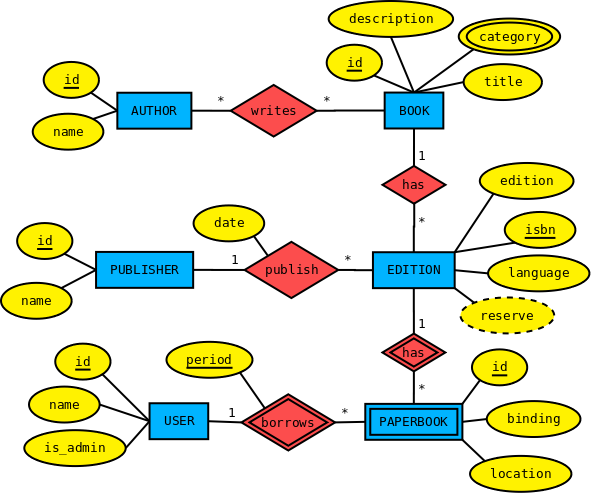
\includegraphics{images/ERDiagram.png}}
\caption{Διάγραμμα οντοτήτων - συσχετίσεων}
\label{fig:ER:diagram}
\end{center}
\end{figure}
\end{landscape}

\subsection{Λογικός σχεδιασμός}

Ο λογικός σχεδιασμός είναι η διαδικασία μετατροπής ενός εννοιολογικού μοντέλου (διαισθητικής περιγραφής) σε τυπικά σχήματα εκφρασμένα στο επιλεγμένο (υποστηριζόμενο από το ΣΔΒΔ) μοντέλο δεδομένων (π.χ. Σχεσιακό μοντέλο) \cite{theodoridis_class_notes}.


(Μήπως εδώ να βάλουμε και τα διαγράμματα component και deployment)

\subsection{Μετατροπή μοντέλου οντοτήτων - συσχετίσεων σε σχεσιακό σχή\-μα}

Οι κανόνες που χρησιμοποιούνται για την μετατροπή του μοντέλου οντοτήτων - συσχετίσεων σε σχεσιακό σχήμα φαίνονται παρακάτω \cite{theodoridis_class_notes}:

\begin{description}

  \item[Οντότητες:] Ένα ισχυρό σύνολο οντοτήτων μετατρέπεται σε πίνακα (με τα ίδια χαρακτηριστικά). Ένα αδύναμο σύνολο οντοτήτων γίνεται πίνακας που περιλαμβάνει μια στήλη για το πρωτεύον κλειδί του ισχυρότερου συνόλου οντοτήτων που το ταυτοποιεί. 
  \item[Συσχετίσεις 1:1 :] Οι συσχετίσεις 1:1 μπορούν να αναπαρασταθούν είτε προσθέτοντας το πρωτεύον κλειδί της μία πλευράς ως επιπλέον χαρακτηριστικό στον πίνακα της άλλη πλευράς είτε δημιουργώντας ένα νέο πίνακα που έχει τα κλειδιά των δύο πινάκων.
  \item[Συσχετίσεις 1:Ν :] Οι συσχετίσεις 1:Ν μπορούν να αναπαρασταθούν απλά με την προσθήκη ενός επιπλέον χαρακτηριστικού στην πλευρά Ν (το πρωτεύον κλειδί τις πλευράς 1). Εάν η συμμετοχή στην πλευρά Ν είναι μερική, μπορεί να προκύψει μία στήλη που να έχει πολλές κενές τιμές. Οπότε η δημιουργία ενός νέου πίνακα μπορεί να συμφέρει.
  \item[Συσχετίσεις Μ:Ν :] Ένα σύνολο συσχετίσεων M:N αναπαριστάται ως πίνακας με στήλες για τα πρωτεύοντα κλειδιά των οντοτήτων που συμμετέχουν, και επιπλέον όλα τα χαρακτηριστικά του συνόλου συσχετίσεων. 
  \item[Σύνθετα χαρακτηριστικά :] Τα σύνθετα χαρακτηριστικά μετατρέπονται σε ένα σύνολο απλών.
  \item[Πλειότιμα χαρακτηριστικά :] Από τα πλειότιμα χαρακτηριστικά ενός συνόλου οντοτήτων προκύπτει νέος πίνακας. Ο πίνακας αυτός έχεις ως στήλες το πρωτεύον κλειδί του συνόλου οντοτήτων και μία ακόμα που αντιστοιχεί στο πλειότιμο χαρακτηριστικό.
  \item[Εξειδίκευση :] Όταν έχουμε εξειδίκευση, τότε προκύπτει ένας πίνακας για κάθε εμπλεκόμενο σύνολο οντοτήτων, όπου καθένας από τους πίνακες εξειδίκευσης συμπεριλαμβάνει ως στήλη το πρωτεύον κλειδί του πίνακα γενίκευσης.
 
\end{description}

Ακολουθώντας τους παραπάνω κανόνες προκύπτει το σχήμα \ref{fig:RelationalModel:diagram}.

\begin{landscape}
\begin{figure}
\begin{center}
\resizebox*{23.5cm}{!}{
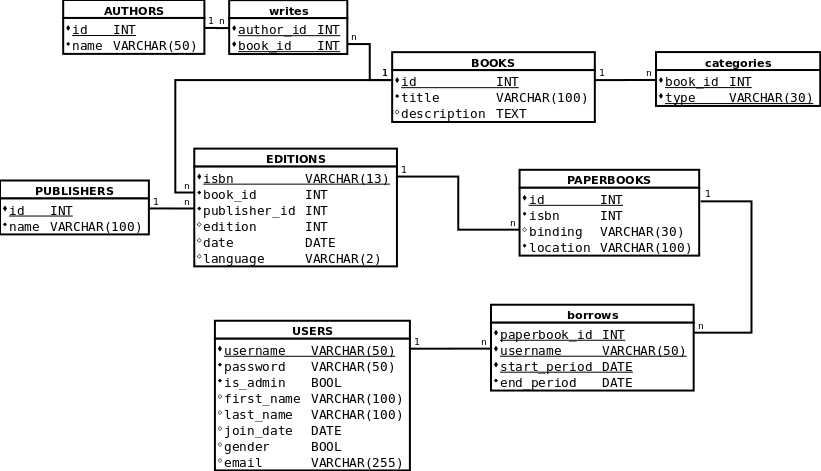
\includegraphics{images/RelationalModel.png}}
\caption{Σχεσιακό σχήμα}
\label{fig:RelationalModel:diagram}
\end{center}
\end{figure}
\end{landscape}


\subsection{Δημιουργία ειδικού χρήστη}

Σαν πρώτο βήμα είναι η δημιουργία ειδικού χρήστη για την βάση έτσι ώστε να μην χρησιμοποιούμε συνέχεια τον υπερχρήστη. Για την επίτευξη αυτού του σκοπού πληκτρολογούμε στο terminal τα παρακάτω: 

\begin{minted}{bash}
$ mysql --user=root --password
Enter password: 
\end{minted} 
%%$

Και αφού έχουμε μπει στην βάση δημιουργούμε ένα καινούργιο χρήστη και μία νέα βάση και δίνουμε στον χρήστη την δυνατότητα να την τροποποιεί. Όλα αυτά επιτυγχάνονται με τα παρακάτω:

\captionof{listing}{Δημιουργία της βάσης δεδομένων}
\begin{minted}[breaklines=true, frame=lines, framesep=2mm, baselinestretch=1.2, fontsize=\footnotesize, linenos]{mysql}
MariaDB [(none)]> CREATE USER 'tme119'@'localhost' IDENTIFIED BY 'tme119_password' ;
MariaDB [(none)]> GRANT USAGE ON *.* TO 'tme119'@'localhost' IDENTIFIED BY 'tme119_password' WITH MAX_QUERIES_PER_HOUR 0 MAX_CONNECTIONS_PER_HOUR 0 MAX_UPDATES_PER_HOUR 0 MAX_USER_CONNECTIONS 0 ;
MariaDB [(none)]> CREATE DATABASE `tme119` CHARACTER SET utf8 COLLATE utf8_general_ci;
MariaDB [(none)]> GRANT ALL PRIVILEGES ON `tme119`.* TO 'tme119'@'localhost';
\end{minted}

Ο λόγος για τον οποίο δημιουργούμε έναν καινούργιο χρήστη είναι για λόγους ασφαλείας έτσι ώστε να μην χρησιμοποιούμε συνέχεια τον υπερχρήστη. Ακόμα στην νέα βάση προτιμήθηκε να χρησιμοποιηθεί το utf8 έτσι ώστε η βάση μας να υποστηρίζει και τα ελληνικά. Μετά την δημιουργία του καινούργιου χρήστη ξαναμπαίνουμε στο ΣΔΒΔ χρησιμοποιώντας τον καινούργιο χρήστη:

\begin{minted}{bash}
$ mysql --user=tme119 --password
Enter password: 
\end{minted} 

%%$

Παρατηρούμε ότι στις μόνες βάσεις που έχει πρόσβαση ο συγκεκριμένος χρήστης είναι η βάση που δημιουργήσαμε πριν και η βάση που είναι δημιουργημένη από την MariaDB και περιέχει πληροφορίες για την βάση.

\begin{minted}[breaklines=true]{mysql}
MariaDB [(none)]> show databases;
+--------------------+
| Database           |
+--------------------+
| information_schema |
| tme119             |
+--------------------+
2 rows in set (0.00 sec)
\end{minted}

\subsection{Δημιουργία πινάκων}


%\begin{landscape}
%\begin{table}[htbp]
%\begin{center}
%  \begin{tabular}{|c|c|m{0.35\textwidth}|m{0.35\textwidth}|m{2.2cm}|c|m{1.5cm}|}
%    \hline
%    {\bf Πεδίο} & {\bf Τύπος μεταβλητής} & {\bf Εύρος τιμών} & {\bf Περιγραφή} & {\bf Πρωτεύον κλειδί} & {\bf Null} & {\bf Ξένο κλειδί} \\ \hline
%    username & VARCHAR(50) & Όλα τα Αλφαριθμητικά ως 50 χαρακτήρες & Ο κωδικός τους χρήστη σε \en{MD5 Hash} & ΟΧΙ & ΟΧΙ & ΟΧΙ \\ \hline
%    password & VARCHAR(50) & Όλα τα Αλφαριθμητικά ως 50 χαρακτήρες & Ο κωδικός τους χρήστη σε \en{MD5 Hash} & ΟΧΙ & ΟΧΙ & ΟΧΙ \\ \hline
%    first\_name & VARCHAR(100) & Όλα τα Αλφαριθμητικά ως 100 χαρακτήρες & Το όνομα του χρήστη & ΟΧΙ & ΝΑΙ & ΟΧΙ \\ \hline
%    last\_name & VARCHAR(100) & Όλα τα Αλφαριθμητικά ως 100 χαρακτήρες & Το επίθετο του χρήστη & ΟΧΙ & ΝΑΙ & ΟΧΙ \\ \hline
%    join\_date & DATE & 1000-01-01 έως 9999-12-31 & Ημερομηνία εγγραφής του χρήστη & OXI & ΝΑΙ & ΟΧΙ \\ \hline
%    gender & BOOL & 0 ή 1 & Το φύλο του χρήστη(Το 1 υποδηλώνει άνδρα και το 0 γυναίκα) & OXI & ΝΑΙ & ΟΧΙ \\ \hline
%    email & VARCHAR(255) & Όλα τα Αλφαριθμητικά ως 255 χαρακτήρες & Το email του χρήστη & ΟΧΙ & ΝΑΙ & ΟΧΙ \\ \hline
%  \end{tabular}
%\caption{Ο πίνακας users.}
%\label{table:db_table:users}
%\end{center}
%\end{table}
%\end{landscape}


\captionof{listing}{Δημιουργία του πίνακα users}
\begin{minted}[breaklines=true, frame=lines, framesep=2mm, baselinestretch=1.2, fontsize=\footnotesize, linenos]{mysql}
MariaDB [book]> CREATE TABLE users (uid INT PRIMARY KEY AUTO_INCREMENT, username VARCHAR(30) UNIQUE NOT NULL, password VARCHAR(50) NOT NULL, is_admin BOOL NOT NULL, first_name VARCHAR(100), last_name VARCHAR(100), join_date DATE, gender BOOL, email VARCHAR(255));

Query OK, 0 rows affected (0.06 sec)

MariaDB [tme119]> describe users;
+------------+--------------+------+-----+---------+----------------+
| Field      | Type         | Null | Key | Default | Extra          |
+------------+--------------+------+-----+---------+----------------+
| uid        | int(11)      | NO   | PRI | NULL    | auto_increment |
| username   | varchar(30)  | NO   | UNI | NULL    |                |
| password   | varchar(50)  | NO   |     | NULL    |                |
| is_admin   | tinyint(1)   | NO   |     | NULL    |                |
| first_name | varchar(100) | YES  |     | NULL    |                |
| last_name  | varchar(100) | YES  |     | NULL    |                |
| join_date  | date         | YES  |     | NULL    |                |
| gender     | tinyint(1)   | YES  |     | NULL    |                |
| email      | varchar(255) | YES  |     | NULL    |                |
+------------+--------------+------+-----+---------+----------------+
9 rows in set (0.00 sec)

MariaDB [tme119]> INSERT INTO users(username,password,is_admin,first_name,last_name,join_date,gender,email) VALUES('anagno',MD5('anagno'),1,'Vasilis','Anagnostopoulos','2015-02-15',1,'anagnwstopoulos@hotmail.com');
Query OK, 1 row affected (0.02 sec);
\end{minted}

\captionof{listing}{Δημιουργία του πίνακα books}
\begin{minted}[breaklines=true, frame=lines, framesep=2mm, baselinestretch=1.2, fontsize=\footnotesize, linenos]{mysql}
MariaDB [book]> CREATE TABLE books (id int UNSIGNED NOT NULL AUTO_INCREMENT, title VARCHAR(100) NOT NULL, description TEXT NOT NULL, PRIMARY KEY (id));

Query OK, 0 rows affected (0.12 sec)

MariaDB [tme119]> describe books;
+-------------+------------------+------+-----+---------+----------------+
| Field       | Type             | Null | Key | Default | Extra          |
+-------------+------------------+------+-----+---------+----------------+
| id          | int(10) unsigned | NO   | PRI | NULL    | auto_increment |
| title       | varchar(100)     | NO   |     | NULL    |                |
| description | text             | NO   |     | NULL    |                |
+-------------+------------------+------+-----+---------+----------------+
3 rows in set (0.01 sec)
\end{minted}

\captionof{listing}{Δημιουργία του πίνακα categories}
\begin{minted}[breaklines=true, frame=lines, framesep=2mm, baselinestretch=1.2, fontsize=\footnotesize, linenos]{mysql}
MariaDB [book]> CREATE TABLE categories (book_id INT UNSIGNED NOT NULL, type VARCHAR(30), PRIMARY KEY (book_id,type), FOREIGN KEY (book_id) REFERENCES books(id) ON DELETE CASCADE ON UPDATE CASCADE);
Query OK, 0 rows affected (0.08 sec)

MariaDB [tme119]> describe categories;
+---------+------------------+------+-----+---------+-------+
| Field   | Type             | Null | Key | Default | Extra |
+---------+------------------+------+-----+---------+-------+
| book_id | int(10) unsigned | NO   | PRI | NULL    |       |
| type    | varchar(30)      | NO   | PRI |         |       |
+---------+------------------+------+-----+---------+-------+
2 rows in set (0.00 sec)
\end{minted}

\captionof{listing}{Δημιουργία του πίνακα authors}
\begin{minted}[breaklines=true, frame=lines, framesep=2mm, baselinestretch=1.2, fontsize=\footnotesize, linenos]{mysql}
MariaDB [book]> CREATE TABLE authors (id INT UNSIGNED NOT NULL AUTO_INCREMENT, name VARCHAR(50) NOT NULL, PRIMARY KEY (id));
Query OK, 0 rows affected (0.08 sec)

MariaDB [tme119]> describe authors;
+-------+------------------+------+-----+---------+----------------+
| Field | Type             | Null | Key | Default | Extra          |
+-------+------------------+------+-----+---------+----------------+
| id    | int(10) unsigned | NO   | PRI | NULL    | auto_increment |
| name  | varchar(50)      | NO   |     | NULL    |                |
+-------+------------------+------+-----+---------+----------------+
2 rows in set (0.00 sec)

\end{minted}


\captionof{listing}{Δημιουργία του πίνακα writes}
\begin{minted}[breaklines=true, frame=lines, framesep=2mm, baselinestretch=1.2, fontsize=\footnotesize, linenos]{mysql}
MariaDB [book]> CREATE TABLE writes (author_id INT UNSIGNED NOT NULL, book_id INT UNSIGNED NOT NULL, PRIMARY KEY (author_id, book_id), FOREIGN KEY (book_id) REFERENCES books(id) ON DELETE CASCADE ON UPDATE CASCADE, FOREIGN KEY (author_id) REFERENCES authors(id) ON DELETE CASCADE ON UPDATE CASCADE);
Query OK, 0 rows affected (0.06 sec)

MariaDB [tme119]> describe writes;
+-----------+------------------+------+-----+---------+-------+
| Field     | Type             | Null | Key | Default | Extra |
+-----------+------------------+------+-----+---------+-------+
| author_id | int(10) unsigned | NO   | PRI | NULL    |       |
| book_id   | int(10) unsigned | NO   | PRI | NULL    |       |
+-----------+------------------+------+-----+---------+-------+
2 rows in set (0.01 sec)
\end{minted}

\captionof{listing}{Δημιουργία του πίνακα publishers}
\begin{minted}[breaklines=true, frame=lines, framesep=2mm, baselinestretch=1.2, fontsize=\footnotesize, linenos]{mysql}
MariaDB [book]> CREATE TABLE publishers ( id INT UNSIGNED NOT NULL AUTO_INCREMENT, name VARCHAR(50) NOT NULL, PRIMARY KEY (id));
Query OK, 0 rows affected (0.03 sec)

MariaDB [tme119]> describe publishers;
+-------+------------------+------+-----+---------+----------------+
| Field | Type             | Null | Key | Default | Extra          |
+-------+------------------+------+-----+---------+----------------+
| id    | int(10) unsigned | NO   | PRI | NULL    | auto_increment |
| name  | varchar(50)      | NO   |     | NULL    |                |
+-------+------------------+------+-----+---------+----------------+
2 rows in set (0.00 sec)
\end{minted}

\captionof{listing}{Δημιουργία του πίνακα editions}
\begin{minted}[breaklines=true, frame=lines, framesep=2mm, baselinestretch=1.2, fontsize=\footnotesize, linenos]{mysql}
MariaDB [book]> CREATE TABLE editions ( isbn VARCHAR(50) UNIQUE NOT NULL, book_id INT UNSIGNED NOT NULL, publisher_id INT UNSIGNED NOT NULL,  edition INT UNSIGNED, date DATE, language VARCHAR(2), PRIMARY KEY (isbn),FOREIGN KEY (book_id) REFERENCES books(id) ON DELETE CASCADE ON UPDATE CASCADE, FOREIGN KEY (publisher_id) REFERENCES publishers(id) ON DELETE CASCADE ON UPDATE CASCADE);
Query OK, 0 rows affected (0.09 sec)

MariaDB [tme119]> describe editions;
+--------------+------------------+------+-----+---------+-------+
| Field        | Type             | Null | Key | Default | Extra |
+--------------+------------------+------+-----+---------+-------+
| isbn         | varchar(50)      | NO   | PRI | NULL    |       |
| book_id      | int(10) unsigned | NO   | MUL | NULL    |       |
| publisher_id | int(10) unsigned | NO   | MUL | NULL    |       |
| edition      | int(10) unsigned | YES  |     | NULL    |       |
| date         | date             | YES  |     | NULL    |       |
| language     | varchar(2)       | YES  |     | NULL    |       |
+--------------+------------------+------+-----+---------+-------+
6 rows in set (0.00 sec)
\end{minted}

\captionof{listing}{Δημιουργία του πίνακα paperbooks}
\begin{minted}[breaklines=true, frame=lines, framesep=2mm, baselinestretch=1.2, fontsize=\footnotesize, linenos]{mysql}
MariaDB [book]> CREATE TABLE paperbooks (id INT UNSIGNED NOT NULL AUTO_INCREMENT,isbn VARCHAR(50) NOT NULL, binding VARCHAR(30), location VARCHAR(100), PRIMARY KEY (id), FOREIGN KEY (isbn) REFERENCES editions(isbn) ON DELETE CASCADE ON UPDATE CASCADE);
Query OK, 0 rows affected (0.04 sec)

MariaDB [tme119]> describe paperbooks;
+----------+------------------+------+-----+---------+----------------+
| Field    | Type             | Null | Key | Default | Extra          |
+----------+------------------+------+-----+---------+----------------+
| id       | int(10) unsigned | NO   | PRI | NULL    | auto_increment |
| isbn     | varchar(50)      | NO   | MUL | NULL    |                |
| binding  | varchar(30)      | YES  |     | NULL    |                |
| location | varchar(100)     | YES  |     | NULL    |                |
+----------+------------------+------+-----+---------+----------------+
4 rows in set (0.00 sec)
\end{minted}

\captionof{listing}{Δημιουργία του πίνακα borrows}
\begin{minted}[breaklines=true, frame=lines, framesep=2mm, baselinestretch=1.2, fontsize=\footnotesize, linenos]{mysql}
MariaDB [book]> CREATE TABLE borrows (paperbook_id INT UNSIGNED NOT NULL,username VARCHAR(50) NOT NULL, start_period DATE NOT NULL, end_period DATE, PRIMARY KEY (paperbook_id, username, start_period), FOREIGN KEY (paperbook_id) REFERENCES paperbooks(id) ON DELETE CASCADE ON UPDATE CASCADE, FOREIGN KEY (username) REFERENCES users(username) ON DELETE CASCADE ON UPDATE CASCADE);
Query OK, 0 rows affected (0.04 sec)

MariaDB [tme119]> describe borrows;
+--------------+------------------+------+-----+---------+-------+
| Field        | Type             | Null | Key | Default | Extra |
+--------------+------------------+------+-----+---------+-------+
| paperbook_id | int(10) unsigned | NO   | PRI | NULL    |       |
| username     | varchar(50)      | NO   | PRI | NULL    |       |
| start_period | date             | NO   | PRI | NULL    |       |
| end_period   | date             | YES  |     | NULL    |       |
+--------------+------------------+------+-----+---------+-------+
4 rows in set (0.00 sec)

\end{minted}





\section{Ανάλυση και Σχεδίαση}

\subsection{Περιπτώσεις χρήσης και διαγράμματα περιπτώσεων χρήσης}

Όπως αναφέρθηκε και στην ενότητα \ref{subsubsection: business_use_case} τα διαγράμματα περιπτώσεων - χρήσης (αγγλ. \en{Use Case Diagrams}) περιγράφουν τη συμπεριφορά ενός συστήματος από την οπτική γωνία ενός χρήστη. (Βάλε το Use case diagramm )

\subsection{Διαγράμματα αλληλεπίδρασης (συνεργασίας και σειράς)}

Τα διαγράµµατα συνεργασίας παρουσιάζουν την αλληλεπίδραση των αντικειµένων µέσω της ανταλλαγής µηνυµάτων και περιγράφουν τη ροή του ελέγχου µέσα στο σύστηµα.
(Βάλε το collaboration diagramm για rent και return book)

Τα διαγράμματα σειράς αναπαριστούν αλληλεπιδράσεις ανάμεσα στα αντικείμενα από μία χρονική άποψη. Η αναπαράσταση επικεντρώνεται στην έκφραση των αλληλεπιδράσεων. Οι συμβολισμοί που χρησιμοποιούνται στα διαγράμματα σειράς φαίνονται στον πίνακα \ref{table:uml_sequence}.

\begin{table}
\begin{center}
  \begin{tabular}{|m{0.20\textwidth}|m{0.60\textwidth}|}
    \hline
     \vspace{0.3cm}
     \resizebox*{0.20\textwidth}{!}{
     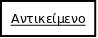
\includegraphics{images/sequence_object.png}}
     & Αντικείμενο. Ένα αντικείμενο αναπαριστάται με ένα ορθογώνιο και μία κάθετη γραμμή, που καλείται γραμμή ζωής του αντικειμένου \cite{virvou_uml}. \\ \hline

     %\vspace{0.3cm}
     \center{
     \resizebox*{!}{0.20\textwidth}{
     
\includegraphics{images/sequence_lifeline.png}}}
     & Ενεργοποίηση αντικειμένου. Μία ενεργοποίηση ανταποκρίνεται στο χρόνο κατά την διάρκεια του οποίου ένα αντικείμενο εκτελεί μία ενέργεια, είτε απευθείας ή μέσω άλλου αντικειμένου, που το χρησιμοποιεί σαν ημισυμβαλλόμενο. Οι ενεργοποιήσεις αναπαριστώνται με ορθογώνιες ράβδους, που τοποθετούνται κατά μήκος των γραμμών ζωής. Η αρχή και το τέλος μίας ράβδου ανταποκρίνεται αντίστοιχα στην αρχή και το τέλος μίας ενεργοποίησης \cite{virvou_uml}. \\ \hline

     \vspace{0.3cm}
     \resizebox*{0.20\textwidth}{!}{
     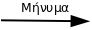
\includegraphics{images/sequence_message.png}}
     & Συγχρονισμένο Μηνύματα. Τα αντικείμενα επικοινωνούν ανταλλάσσοντας μηνύματα, τα οποία αναπαριστώνται με οριζόντια βέλη σχεδιασμένα από τον αποστολέα του μηνύματος προς τον παραλήπτη του μηνύματος \cite{virvou_uml}. Επειδή είναι συγχρονισμένα, θα πρέπει να περιμένει να τελειώσει η διαδικασία πριν προχωρήσει στην επόμενη \\ \hline

     \vspace{0.3cm}
     \resizebox*{0.20\textwidth}{!}{
     
\includegraphics{images/sequence_return.png}}
     & Επιστροφή. Βέλος επιστροφής μηνύματος. \\ \hline

  \end{tabular}
\caption{Τα εικονίδια του διαγράμματος σειράς.}
\label{table:uml_sequence}
\end{center}
\end{table}

(Εδώ βάλε το διάγραμμα σειράς!)

Οι πιο σημαντική αλληλεπίδραση του πληροφοριακού μας συστήματος είναι ενοικίαση των βιβλίων και γι` αυτό το λόγο αναπαριστάται και σε διάγραμμα σειράς. Όπως φαίνεται και στο διάγραμμα σειράς στο σχήμα \ref{fig:sequence_ticket}???? ο πελάτης για να ενοικιάσει  κάποιο βιβλίο θα πρέπει πρώτα να συνδεθεί με το πληροφοριακό σύστημα. Εφόσον τα στοιχεία του είναι σωστά προχωρά η διαδικασία της επιλογής. Έπειτα επιλέγει το βιβλίο που θέλει και εφόσον είναι διαθέσιμο  ολοκληρώνεται η διαδικασία με την παραλαβή του αντιτύπου.

%\begin{landscape}
%\begin{figure}
%\begin{center}
%\resizebox*{!}{\textwidth}{
%\includegraphics{images/sequence_ticket.png}}
%\caption{Διάγραμμα σειράς για την αγορά εισητηρίου}?????
%\label{fig:sequence_ticket}
%\end{center}
%\end{figure}
%\end{landscape}

\subsection{Διάγραμμα Βασικών κλάσεων πεδίου Εφαρμογής}?????????

%\begin{landscape}
%\begin{figure}
%\begin{center}
%\resizebox*{!}{\textwidth}{
%\includegraphics{images/class_diagramm.jpg}}
%\caption{Το διάγραμμα κλάσεων}
%\label{fig:class_diagramm}
%\end{center}
%\end{figure}
%\end{landscape}


\subsection{Αναλυτικά διαγράμματα κλάσεων συνοδευμένα από OCL περιορισμούς}?????????

\subsection{Διαγράμματα Επικοινωνίας και Αλληλεπίδρασης}???????? Αυτά νομίζω ότι δεν χρειάζονται...




%ΔΕΝ ΧΡΕΙΑΖΟΝΤΑΙ
%\section{Μοντέλο Οντοτήτων-Συσχετίσεων της Βάσεις Δεδομένων του Πληροφοριακού Συστήματος}

%Στην ενότητα αυτή δίνεται η περιγραφή του μοντέλου Οντοτήτων-Συσχετίσεων (αγγλ. \en{Entity-Relationship Diagram} από το οποίο υλοποιείται το Σχεσιακό Διάγραμμα της Βάσης Δεδομένων του Πληροφοριακού Συστήματος.

%\subsection{Περιγραφή Οντοτήτων}
%\label{entity}

%Οι βασικές οντότητες είναι οι παρακάτω:

%\begin{description}
%\item test
%\end{description}

%\subsection{Περιγραφή Σχέσεων}
%\label{relationship}

%Οι βασικές σχέσεις είναι οι παρακάτω:

%\subsection{ER διάγραμμα του Πληροφοριακού Συστήματος}

%Οι ενότητες \ref{entity} και \ref{relationship} απεικονίζονται στο σχήμα \ref{}.

\phantomsection \label{Βιβλιογραφία}
\addcontentsline{toc}{section}{Βιβλιογραφία}
%\mtcaddchapter[Βιβλιογραφία] % Λόγω του minitoc
\bibliographystyle{plain}
\bibliography{references}

\newpage

\end{document}

